\chapter{Introducción}
\label{chap:introduccion}

\drop{S}{  olamente} en 2018, el \textbf{Museo Reina Sofía} de Madrid recibió 3,9 millones de visitantes, aproximadamente un 2\% más que el año anterior. Del mismo modo, el \textbf{Museo de Prado} recibió casi 3 millones, un 2,4\% más que en 2017. Otro ejemplo de esto es el \textbf{Macba}, el Museo de Arte Contemporáneo de Barcelona, que recibió en 2018 casi 332,000 visitantes, un 28\% más que el año anterior\footnote{\url{https://www.abc.es/cultura/arte/abci-museos-espanoles-crecen-2018-201901021635_noticia.html}}. Con estos datos, puede verse que el interés por los museos está creciendo cada vez más.

Pero la industrias de ocio que indiscutible más dinero genera es la \textbf{industria de videojuegos}, que solo en 2018 generó 43 mil millones de dólares, un 18\% más que en 2017\footnote{\url{https://tcrn.ch/2HtFczS}}. Por dar un contexto de estas cifras, en 2016 la suma conjunta del cine y la música en el mundo \textit{solo} generó 815 millones de dólares\footnote{\url{https://www.elperiodico.com/es/ocio-y-cultura/20180827/videojuegos-cine-musica-cultura-comparativa-7001883}}.

Dado el éxito global de esta industria, han comenzado a nacer nuevas maneras de jugar y nuevas técnicas de interacción con los usuarios, como la \textbf{Realidad Virtual}. La Realidad Virtual es un paradigma de interacción que intenta ofrecer a sus jugadores una experiencia lo más \textbf{inmersiva} posible, para lo que hace uso de la visión estereoscópica de las personas para hacerles creer que el mundo real es lo que ven, y no solo una pantalla.

Además, los dispositivos que permiten hacer uso de estas tecnologías se están abaratando cada vez más, hasta el punto de que un jugador casual puede permitirse adquirir un headset \acs{VR} para utilizarlo esporádicamente, en lugar de ser una tecnología que solo se plantena comprar aquellos que creen que le van a dar mucho uso.

\section{Motivación del proyecto}

El principal objetivo a la hora de integrar videojuegos y tecnologías de Realidad Virtual en este proyecto es el poder crear respectivamente entornos interactivos e inmersivos que, unidos al potencial motivador que tienen de manera intrínseca los videojuegos, consigan animar a los usuarios que disfruten de \MineRVa a visitar museos reales y ser, principalmente para aquellos que no puedan hacerlo por razones físicas, un sustituto que les permita disfrutar en la medida de lo posible de ello. 

\section{Motivación personal}

Siempre he estado muy interesado en el desarrollo de videojuegos y en el proceso técnico que hay detrás. Durante el grado, que estudié en la Universidad de Castilla-La Mancha, tuve la suerte de coincidir con algunos profesores que también estaban muy interesados en este tema y que habían organizado dos cursos; el primero, en 2015, fue el \textbf{Curso de Desarrollo de videojuegos multi-plataforma para dispositivos móviles}\footnote{\url{http://www.curso-openfl.cedv.quijost.com/}}, un curso de 100 horas en el que desarrollamos un juego en 2D en Haxe utilizando el framework OpenFL.

Tras él, dos años más tarde completé el \textbf{Curso de Experto en desarrollo de videojuegos}\footnote{\url{http://cedv.es}}, de 750 horas, en el que realizamos varios proyectos en C++ utilizando el motor de gráficos Ogre3D y otras tecnologías como la librería de interfaces CEGUI o el motor de físicas Bullet.

A raíz de estos cursos comencé a interesarme por Blender, un programa de diseño 3D que integra todos los componentes necesarios para modelar, texturizar, animar y renderizar prácticamente cualquier proyectos.

Por un lado, nunca había trabajando con entornos de desarrollo específicos para videojuegos como Unity, y ni mucho menos con tecnologías de Realidad Virtual, lo que me pareció un reto extremadamente interesante. Por otro, aunque ya había trabajado desarrollando sistemas interactivos nunca lo había hecho aplicando metodologías adecuadas y específicas de desarrollo de videojuegos, por lo que este proyecto parecía el contexto perfecto como primera toma de contacto con ellas.

Del mismo modo, siempre me ha interesado mucho la Historia del Arte y he intentado visitar museos siempre que he tenido la oportunidad, por lo que estoy muy motivado al poder integrar ambos en este proyecto.

\section{Entorno}

El entorno de ejecución de \MineRVa está compuesto por unas gafas de Realidad Virtual, dos controladores y un ordenador personal. Por tanto, el programa final debe ser lo suficientemente ligero y eficiente en cuanto a recursos para poder ser ejecutado en un ordenador que no sea especialmente potente.

La figura \ref{fig:entorno}, renderizada en Blender, presenta un ejemplo de ejecución en el que se puede ver a un usuario llevando puestos el headset \acs{VR} y los mandos mientras juega en uno de las escenarios iniciales. 

\begin{figure}[!h]
\vspace{0.4cm}
\begin{center}
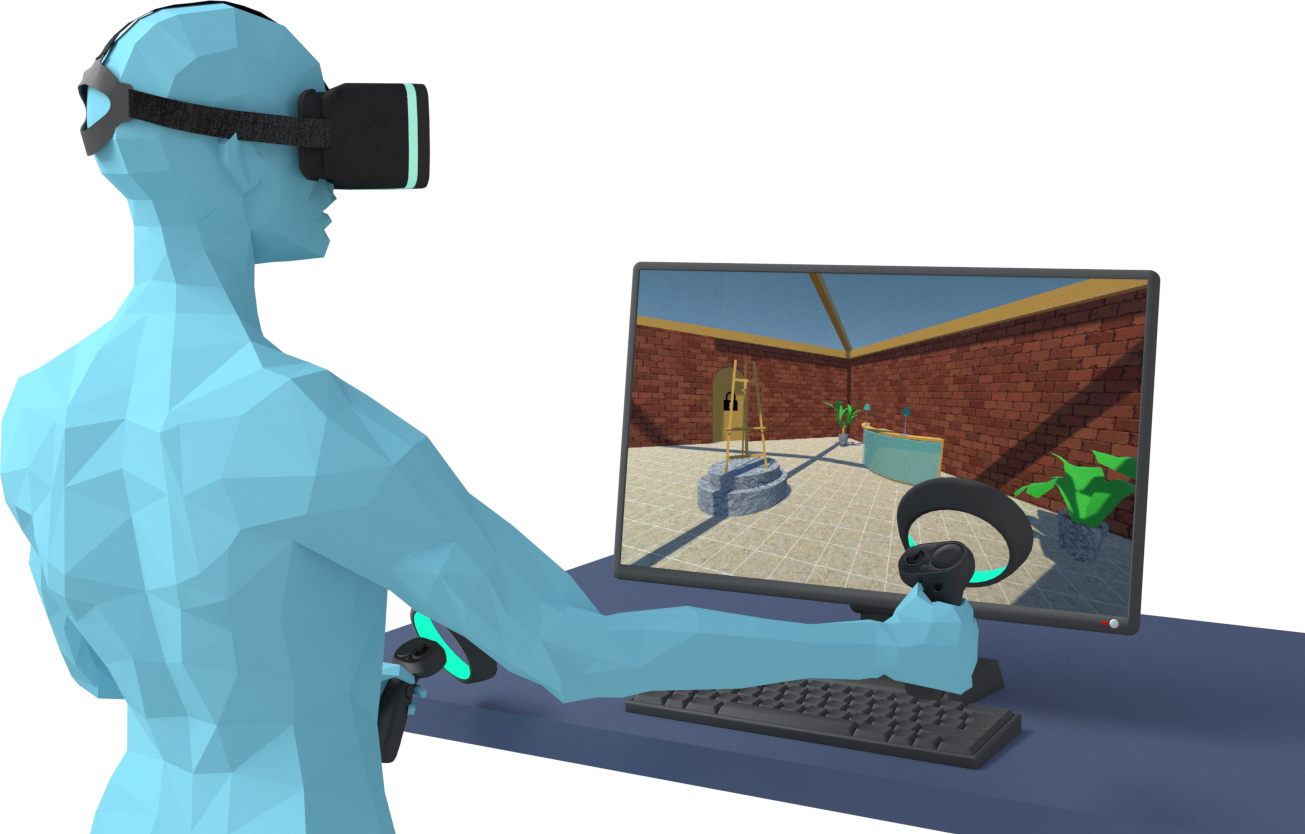
\includegraphics[width=1\textwidth]{imagenes/1/entorno-diffuse-2.png}
\caption{Diagrama de entorno de \MineRVa}
\label{fig:entorno}
\end{center}
\end{figure}

Además, como en este juego no es necesario hacer movimientos rápidos y bruscos, no es necesario contar con mucho espacio libre alrededor del jugador, lo que lo hace aún más accesible al público en general, que no tendrá que disponer de una sala amplia específica para utilizar tecnologías \acs{VR}.


\section{Objetivos}

\subsection{Objetivo principal}

El objetivo de \MineRVa es crear una experiencia inmersiva en la que el jugador se sienta gratificado al ir resolviendo los pequeños acertijos que se le proponen. Con ello se pretende alcanzar dos objetivos diferentes; por un lado, se busca conseguir que nativos digitales que no suelan visitar museos encuentren en \MineRVa una excusa para hacerlo de manera divertida, y por el otro que usuarios más mayores a los que les gusta visitarlos encuentre en la temática de este proyecto una excusa para jugarlo y disfrutar de la misma forma. En cualquiera de los dos casos se espera que, tras completar el juego, la mayoría de usuarios se interesen en visitar museos reales.

Por otro lado, uno de los nichos de jugadores más pequeños y a la vez uno en el que más se ha pensado es en aquellas personas con movilidad reducida que físicamente no pueden visitar museos. Se espera ayudar especialmente a este colectivo consiguiendo una experiencia equivalente en la medida de lo posible, además de intentar hacerla más amena y motivadora enmarcándola en el contexto de un videojuego.

\subsection{Objetivos secundarios}

Como objetivos secundarios, de naturaleza más personal, se presenta el aprender a desarrollar programas basados en tecnologías de Realidad Virtual, así como a elegir y configurar un entorno adecuado para ello.

Además, al estudiar metodologías de desarrollo de videojuegos reales se espera obtener un mejor conocimiento de cómo funciona el desarrollo de un proyecto de estas características.

\section{Estructura del documento}

Este documento ha sido estructurado siguiendo la normativa de \acs{TFM} de la Escuela Técnica Superior de Ingenierías Informática y de Telecomunicación de la Universidad de Granada a través de los siguientes capítulos.

\subsubsection{Capítulo \ref{chap:estado_arte}. \nameref{chap:estado_arte}}

En este capítulo se realiza una presentación del estado actual de las áreas tratadas en este \acs{TFM}, recopilando y exponiendo información relevante relacionada con la Realidad Virtual o el Desarrollo de Videojuegos, entre otros.

\subsubsection{Capítulo \ref{chap:analisis_problema}. \nameref{chap:analisis_problema}}

En este capítulo se introduce este proyecto y se hablará de la concepción inicial y de la narrativa de \textit{MineRVa}.

\subsubsection{Capítulo \ref{chap:tecnologia}. \nameref{chap:tecnologia}}

Este capítulo recoge los recursos tanto hardware como software que se han utilizado para el desarrollo y documentación de este proyecto.

\subsubsection{Capítulo \ref{chap:metodologias}. \nameref{chap:metodologias}}

A lo largo de este capítulo se hablará de las metodologías de desarrollo de videojuegos y se presentarán las metodologías de trabajo y desarrollo seguidas a lo largo de este proyecto.

\subsubsection{Capítulo \ref{chap:plan_entregas}. \nameref{chap:plan_entregas}}

En este capítulo se presenta y detalla el plan de entregas llevado a cabo al inicio del proyecto para poder cumplir con el plazo de tiempo de entrega.

\subsubsection{Capítulo \ref{chap:desarrollo}. \nameref{chap:desarrollo}}

A lo largo de esta capítulo se presenta el trabajo realizado en el marco del plan de entregas del proyecto, además de los resultados obtenidos y los principales problemas encontrados.

\subsubsection{Capítulo \ref{chap:conclusiones}. \nameref{chap:conclusiones}}

En este capítulo se presenta el resultado final del proyecto, las conclusiones extraídas de su desarrollo y se proponen unas líneas de trabajo futuro para continuar con este proyecto.